\documentclass[spanish,a4paper,14pt,oneside]{extreport}
 
  %%%%%%%%%%%%%%%%%%%%%%%%%%%%%%%%%%%%%%%%%%%%%%%%%%%%%%%%%%%%%%%%%%%%%%%%%%%%%%%
  \usepackage[dvips]{graphicx}
  \usepackage[dvips]{epsfig}
  \usepackage[utf8]{inputenc}
  \usepackage[spanish]{babel}
  \usepackage{alltt}
  \usepackage{algorithm}
  \usepackage{algorithmic}
  \usepackage{multirow}
  \usepackage[top=2cm, bottom=2cm, left=2cm, right=2cm]{geometry}
   
  %%%%%%%%%%%%%%%%%%%%%%%%%%%%%%%%%%%%%%%%%%%%%%%%%%%%%%%%%%%%%%%%%%%%%%%%%%%%%%%
  \usepackage{array}
  \widowpenalty=5000
  \usepackage{tocloft}
  \renewcommand{\cftchapafterpnum}{\vspace{10pt}}
  \usepackage{eurosym}
  \usepackage[hidelinks]{hyperref}
  \usepackage{breakurl}
  \usepackage{subfig}
  %%%%%%%%%%%%%%%%%%%%%%%%%%%%%%%%%%%%%%%%%%%%%%%%%%%%%%%%%%%%%%%%%%%%%%%%%%%%%%%
   
  \newcommand{\SONY}{{\sc Sony}}
  \newcommand{\MICROSOFT}{{\sc Microsoft}}
  \newcommand{\GCC}{\textsf{\textsc{G}CC}}
  \newcommand{\INTEL}{\textsf{\textsc{I}ntel}}
   
  %%% Traducimos el pseudocodigo
  \renewcommand{\algorithmicwhile}{\textbf{mientras}}
  \renewcommand{\algorithmicend}{\textbf{fin}}
  \renewcommand{\algorithmicdo}{\textbf{hacer}}
  \renewcommand{\algorithmicif}{\textbf{si}}
  \renewcommand{\algorithmicthen}{\textbf{entonces}}
  \renewcommand{\algorithmicrepeat}{\textbf{repetir}}
  \renewcommand{\algorithmicuntil}{\textbf{hasta que}}
  \renewcommand{\algorithmicelse}{\textbf{en otro caso}}
  \renewcommand{\algorithmicfor}{\textbf{para}}
   
  %\newcommand{\RETURN}{\textbf{retornar} }
  \newcommand{\RET}{\STATE \textbf{retornar} }
  \newcommand{\TO}{\textbf{hasta} }
  \newcommand{\AND}{\textbf{y} }
  \newcommand{\OR}{\textbf{o} }
   
  %%%%%%%%%%%%%%%%% Creamos un entorno para listar código fuente %%%%%%%%%%%%%%%
  \newenvironment{sourcecode}
  {\begin{list}{}{\setlength{\leftmargin}{1em}}\item\scriptsize\bfseries}
  {\end{list}}
   
  \newenvironment{littlesourcecode}
  {\begin{list}{}{\setlength{\leftmargin}{1em}}\item\tiny\bfseries}
  {\end{list}}
   
  \newenvironment{summary}
  {\par\noindent\begin{center}\textbf{Abstract}\end{center}\begin{itshape}\par\noindent}
  {\end{itshape}}
   
  \newenvironment{keywords}
  {\begin{list}{}{\setlength{\leftmargin}{1em}}\item[\hskip\labelsep \bfseries Keywords:]}
  {\end{list}}
   
  \newenvironment{palabrasClave}
  {\begin{list}{}{\setlength{\leftmargin}{1em}}\item[\hskip\labelsep \bfseries Palabras clave:]}
  {\end{list}}
   
   
  %%%%%%%%%%%%%%%%%%%%%%%%%%%%%%%%%%%%%%%%%%%%%%%%%%%%%%%%%%%%%%%%%%%%%%%%%%%%%%%
  % Format
  %%%%%%%%%%%%%%%%%%%%%%%%%%%%%%%%%%%%%%%%%%%%%%%%%%%%%%%%%%%%%%%%%%%%%%%%%%%%%%%
  %\usepackage{showframe}
  %\marginparwidth 0mm
  %%\topmargin -4 mm
  %\topmargin -21 mm
  %\headheight 10 mm
  %\headsep 10 mm
   
  %\textheight 229 mm
  %\textheight 246 mm
   
  %\oddsidemargin -5.4 mm
  %\evensidemargin -5.4 mm
  %\oddsidemargin 5 mm
  %\evensidemargin 5 mm
   
  %\oddsidemargin -3 mm
  %\evensidemargin -3 mm
   
  %\textwidth 17 cm
  %\textwidth 15 cm
  %\columnsep 10 mm
   
  \input{amssym.def}
   
  %%%%%%%%%%%%%%%%%%%%%%%%%%%%%%%%%%%%%%%%%%%%%%%%%%%%%%%%%%%%%%%%%%%%%%%%%%%%%%%
   
  \begin{document}
   
  %%%%%%%%%%%%%%%%%%%%%%%%%%%%%%%%%%%%%%%%%%%%%%%%%%%%%%%%%%%%%%%%%%%%%%%%%%%%%%%
  % First Page
  %%%%%%%%%%%%%%%%%%%%%%%%%%%%%%%%%%%%%%%%%%%%%%%%%%%%%%%%%%%%%%%%%%%%%%%%%%%%%%%
   
  \pagestyle{empty}
  \thispagestyle{empty}
   
   
  \newcommand{\HRule}{\rule{\linewidth}{1mm}}
  \setlength{\parindent}{0mm}
  \setlength{\parskip}{2.5mm}
   
  \vspace*{\stretch{0.5}}
   
  \begin{center}
  
\includegraphics[scale=0.8]{images/logo_nuevo}\\[10mm]
  {\Huge Trabajo Fin de Grado}\\
  \bigskip
  {\LARGE Grado en Ingeniería Informática}\\
  \end{center}
   
  \HRule
  \begin{flushright}
         {\Huge Análisis de los resultados de los sistemas de entrenamiento del Pensamiento Computacional} \\[2.5mm]
         {\Large \textit{Analysis of the results of Computational Thinking training systems}} \\[5mm]
         {\Large Samuel Valcárcel Arce} \\[5mm]
  \end{flushright}
  \HRule
  \vspace*{\stretch{2}}
  \begin{center}
   \Large La Laguna, \today
  \end{center}
   
  \setlength{\parindent}{5mm}
   
  %%%%%%%%%%%%%%%%%%%%%%%%%%%%%%%%%%%%%%%%%%%%%%%%%%%%%%%%%%%%%%%%%%%%%%%%%%%%%%%
  % Signature page (add the official stamp)
  %%%%%%%%%%%%%%%%%%%%%%%%%%%%%%%%%%%%%%%%%%%%%%%%%%%%%%%%%%%%%%%%%%%%%%%%%%%%%%%
  \newpage
  %\cleardoublepage
  \thispagestyle{empty}
   
  Dra. Dª {\bf Coromoto Antonia León Hernández}, con N.I.F. 78.605.216-W
  profesora
  Titular de Universidad
  del área
  de Lenguajes y Sistemas Informáticos, adscrita al Departamento de Ingeniería Informática y Sistemas de la Universidad de La Laguna, como tutora,
   
  \bigskip
  Dr. D. {\bf Carlos Segura González}, con N.I.F. 78.704.244-S
  profesor
  Titular
  adscrito al Área
  de Ciencias de la Computación
  del Centro de Investigación Matemática en Guanajuato, México, como cotutor
   
  \bigskip
  \bigskip
  {\bf C E R T I F I C A N}
   
  \bigskip
  \bigskip
  \bigskip
  Que la presente memoria titulada:
   
  \bigskip
  ``{\it Análisis de los resultados de los sistemas de entrenamiento del Pensamiento Computacional}''
   
  \bigskip
  \bigskip
  \bigskip
   
  \noindent ha sido realizada bajo su dirección por D. {\bf Samuel Valcárcel Arce},
  con N.I.F. 54.063.506-M.
   
  \bigskip
  \bigskip
   
  Y para que así conste, en cumplimiento de la legislación vigente y a los efectos
  oportunos firman la presente en La Laguna a \today
   
  %\cleardoublepage
  \newpage
  %%%%%%%%%%%%%%%%%%%%%%%%%%%%%%%%%%%%%%%%%%%%%%%%%%%%%%%%%%%%%%%%%%%%%%%%%%%%%%%
  \thispagestyle{empty}
   
  { \flushright
   
  \begin{LARGE}
  Agradecimientos
  \end{LARGE}
   
  \hspace{3mm}
   
  \begin{large}
   
   
  \hspace{3mm}
    A mi tutora Coromoto León, por guiarme en todas y cada una de las tareas a
    desarrollar durante la realización del Trabajo Fin de Grado, así como resolver cualquier problema relacionado con el proyecto. 
    Y a mi madre por su paciencia y apoyo incondicional durante estos años de estudios en el Grado
    de Ingeniería Informática.
   
   
  \end{large}
   
  }
   
  %%%%%%%%%%%%%%%%%%%%%%%%%%%%%%%%%%%%%%%%%%%%%%%%%%%%%%%%%%%%%%%%%%%%%%%%%%%%%%%%%
  \newpage
   
  \begin{huge}
  Licencia
  \end{huge}
   
  \bigskip
  \begin{center}
  \includegraphics[scale=1.5]{images/by-nc_88x31}\\[10mm]
  {\Large \copyright~Esta obra está bajo una licencia de Creative Commons Reconocimiento-NoComercial 4.0 Internacional.
  }
  \end{center}
   
   
   
  %%%%%%%%%%%%%%%%%%%%%%%%%%%%%%%%%%%%%%%%%%%%%%%%%%%%%%%%%%%%%%%%%%%%%%%%%%%%%%%
  \newpage  %\cleardoublepage
  \begin{abstract}
  {\em
   
  El objetivo del Trabajo Fin de Grado ha consistido en el estudio de diversas plataformas relacionadas con el pensamiento computacional y en qué medida los resultados ayudan a los profesores a conocer si
  los alumnos que lo realizan están aprendiendo nuevos conocimientos.

  Se ha realizado una plataforma, con el fin de complementar los resultados recibidos por el profesorado una vez que el alumnado ha finalizado los tests, de manera que muestre unas estadísticas en forma de gráficos
  filtrados por edades, niveles completados, líneas de código usadas, etc.

  Debido a que esta plataforma actualmente sólo cuenta con acceso por parte de los profesores, pero con las mejoras propuestas podrían entrar también los alumnos, se ha diseñado pensando en la sencilez y comodidad a la hora de usarla. Una vez que el
  profesor introduzca los resultados, podrá también obtener informes generados a través de la aplicación con las estadísticas de sus cursos impartidos.

  }
   
  \begin{palabrasClave}
  Pensamiento Computacional, Plataforma, Aplicación web, Retos, CodeCharts, Estadísticas, Progreso, Ruby.
  \end{palabrasClave}
   
  \end{abstract}
  %%%%%%%%%%%%%%%%%%%%%%%%%%%%%%%%%%%%%%%%%%%%%%%%%%%%%%%%%%%%%%%%%%%%%%%%%%%%%%%
   
  %%%%%%%%%%%%%%%%%%%%%%%%%%%%%%%%%%%%%%%%%%%%%%%%%%%%%%%%%%%%%%%%%%%%%%%%%%%%%%%
  \newpage  %\cleardoublepage
  \begin{summary}
  {\em
   
    The objective of the Final Degree Project has been the study of some platforms related to computer thinking and how the results help teachers to know if
    the students who do it are learning new knowledge.

    A platform has been created  to complement the results received by the faculty once the students have finished the tests, in order to show statistics in the form of graphs
    filtered by ages, levels completed, lines of code used, etc.
    
    Because this platform currently only includes teachers, but with the proposed improvements of students accounts also, it has been designed thinking about the simplicity and 
    comfort when using it. Once the professor inserts the results, you can obtain reports generated too through the application with the statistics of his courses taught.
  }
   
  \begin{keywords}
  Computationa Thinking, Platform, Web app, Challenges, CodeCharts, Stats, Progress, Ruby
  \end{keywords}
   
  \end{summary}
  %%%%%%%%%%%%%%%%%%%%%%%%%%%%%%%%%%%%%%%%%%%%%%%%%%%%%%%%%%%%%%%%%%%%%%%%%%%%%%%
   
  %%%%%%%%%%%%%%%%%%%%%%%%%%%%%%%%%%%%%%%%%%%%%%%%%%%%%%%%%%%%%%%%%%%%%%%%%%%%%%%
  \newpage{\pagestyle{empty}}
  \thispagestyle{empty}
   
  %%%%%%%%%%%%%%%%%%%%%%%%%%%%%%%%%%%%%%%%%%%%%%%%%%%%%%%%%%%%%%%%%%%%%%%%%%%%%%%
   
   
  \pagestyle{myheadings} %my head defined by markboth or markright
  % No funciona bien \markboth sin "twoside" en \documentclass, pero al
  % ponerlo se dan un montón de errores de underfull \vbox, con lo que no se
  % ha puesto.
  \markboth{Samuel Valcárcel Arce}{Análisis de los resultados del entrenamiento del PC}
   
  %%%%%%%%%%%%%%%%%%%%%%%%%%%%%%%%%%%%%%%%%%%%%%%%%%%%%%%%%%%%%%%%%%%%%%%%%%%%%%%
  %Numeracion en romanos
  \renewcommand{\thepage}{\roman{page}}
  \setcounter{page}{1}
   
  %%%%%%%%%%%%%%%%%%%%%%%%%%%%%%%%%%%%%%%%%%%%%%%%%%%%%%%%%%%%%%%%%%%%%%%%%%%%%%%
   
  \tableofcontents
   
  %%%%%%%%%%%%%%%%%%%%%%%%%%%%%%%%%%%%%%%%%%%%%%%%%%%%%%%%%%%%%%%%%%%%%%%%%%%%%%%
  \newpage{\pagestyle{empty}}
   
  \listoffigures
   
  %%%%%%%%%%%%%%%%%%%%%%%%%%%%%%%%%%%%%%%%%%%%%%%%%%%%%%%%%%%%%%%%%%%%%%%%%%%%%%%
  \newpage{\pagestyle{empty}}
   
  \listoftables
   
  %%%%%%%%%%%%%%%%%%%%%%%%%%%%%%%%%%%%%%%%%%%%%%%%%%%%%%%%%%%%%%%%%%%%%%%%%%%%%%%
  \newpage{\pagestyle{empty}}
   
  %%%%%%%%%%%%%%%%%%%%%%%%%%%%%%%%%%%%%%%%%%%%%%%%%%%%%%%%%%%%%%%%%%%%%%%%%%%%%%%
  %Numeracion a partir del capitulo I
  \renewcommand{\thepage}{\arabic{page}}
  \setcounter{page}{1}
   
   
  \chapter{Introducción}
  \label{chapter:intro}
   
  %%%%%%%%%%%%%%%%%%%%%%%%%%%%%%%%%%%%%%%%%%%%%%%%%%%%%%%%%%%%%%%%%%%%%%%%%%%%%
% Chapter 1: Introducción 
%%%%%%%%%%%%%%%%%%%%%%%%%%%%%%%%%%%%%%%%%%%%%%%%%%%%%%%%%%%%%%%%%%%%%%%%%%%%%%%

%---------------------------------------------------------------------------------
\section{Introducción}
\label{1:sec:1}

\begin{itemize}
  \item Item 1 \cite{Bay1}
  \item Item 2
  \item Item 3
  \item Item 4
\end{itemize}

%---------------------------------------------------------------------------------
\section{Antecedentes y estado actual}
\label{1:sec:2}

Para explicar los antecedentes y el estado actual del tema en este proyecto se tendrán en cuenta las referencias citadas a continuación:

\begin{itemize}
  \item En un artículo publicado en 2017 \textit{"Teacher Configurable Coding Challenges for Block Languages"} se explica como una herramienta llamada \textbf{COPPER}\cite{Tumlin:2017:TCC:3017680.3022467}, una herramienta desarrollada para crear puzzles de código en una cuadrícula usando lenguajes de programación basado en bloques, similar a los realizados en la plataforma Code.org "Hour of Code", que tiene el potencial de incrementar el interés y el compromiso con el pensamiento computacional.
  \item En 2015, en la revista llamada \textbf{"ACM INROADS"}, publicó un artículo\cite{Wilson:2015:HCB:2786608.2746406} mencionando la ayuda recibida por la NSF (National Science Foundation), una agencia federal independiente creada por el Congreso de los Estados Unidos en 1950 para promover el progreso de la ciencia, la salud nacional y muchos otros aspectos relevantes para el país, con lo que muchos de los alumnos en colegios sin recursos o estudiantes de color tuvieran acceso a una educación, tanto secundaria como primaria, digna en las Ciencias de la Computación.
  \item Por último, en un artículo\cite{Brown:2016:PFD:2839509.2844661} publicado en 2016, en el libro llamado "Proceedings of the 47th ACM Technical Symposium on Computer Science Education"  se constata que las enseñanzas sobre la Ciencia de la Computación que se componen de actividades que usen la programación basada en bloques, como pueden ser con Scratch, Alice y las "Hour of Code" de Code.org, incentivan tanto a alumnos como profesores a indagar con más profundidad en el mundo del pensamiento computacional.

\end{itemize}

Cabe mencionar que uno de los recursos que usaremos para este proyecto sería su repositorio alojado en la plataforma \textbf{Github}, que supondría una ayuda a la hora de analizar el diseño de la página Code.org, de tal manera que podamos aportar unas estadísticas más concretas de cada alumno.

%---------------------------------------------------------------------------------
\section{Sección Tres}
\label{1:sec:3}

Bla, bla, bla  \ref{1:sec:1}

%---------------------------------------------------------------------------------
\section{Sección Cuatro}
\label{1:sec:4}

Bla, bla, bla

%------------------------------------------------------------------------------
\begin{figure}[!th]
\begin{center}
\includegraphics[width=0.5\textwidth]{images/arbolbinario.eps}
\caption{Ejemplo}
\label{fig:ArbolBinario}
\end{center}
\end{figure}
%------------------------------------------------------------------------------


   
  %%%%%%%%%%%%%%%%%%%%%%%%%%%%%%%%%%%%%%%%%%%%%%%%%%%%%%%%%%%%%%%%%%%%%%%%%%%%%%%
   
  \chapter{Antecedentes y estado actual del tema}
  \label{chapter:Estadodelarte}
   
  %%%%%%%%%%%%%%%%%%%%%%%%%%%%%%%%%%%%%%%%%%%%%%%%%%%%%%%%%%%%%%%%%%%%%%%%%%%%%%%
% Chapter 2: Título del capítulo 2
%%%%%%%%%%%%%%%%%%%%%%%%%%%%%%%%%%%%%%%%%%%%%%%%%%%%%%%%%%%%%%%%%%%%%%%%%%%%%%%

Siguiendo el curso del campus de la biblioteca, haciendo uso de .Q, una herramienta de búsqueda de información de la Universidad de La Laguna, se realizó una búsqueda de artículos relacionados con el Pensamiento Computacional, algunos de ellos de la famosa revista ACM.

%++++++++++++++++++++++++++++++++++++++++++++++++++++++++++++++++++++++++++++++

\section{Estado del arte}
\label{2:sec:1}

Para explicar los antecedentes y el estado actual del tema en este proyecto se tendrán en cuenta las referencias citadas a continuación:

\begin{itemize}
  \item En un artículo\cite{Tumlin:2017:TCC:3017680.3022467} publicado en 2017, \textit{"Teacher Configurable Coding Challenges for Block Languages"}, se explica como una herramienta llamada \textbf{COPPER} (CustOmizable Puzzle Programming EnviRonment), desarrollada para crear puzzles de código en una cuadrícula usando lenguajes de programación basado en bloques, 
  similar a los realizados en la plataforma Code.org "Hour of Code", tiene el potencial de incrementar el interés y el compromiso con el pensamiento computacional. 
  
  De esta manera, se fomenta la forma de pensar computacionalmente a través de tareas que mejoren estas habilidades dentro un ambiente similar a un juego, normalmente fomentando que los estudiantes creen programas que dicten las acciones de un personaje a medida que avanza a través de un nivel de rompecabezas, similares a los de Code.org.

  Este proyecto busca aumentar la utilidad de este tipo de puzzles, permitiendo a los profesores personalizar los elementos visuales y mecánicos de los niveles que necesiten para impartir su contenido. Por ejemplo, un docente que tenga que dar una lección de historia sobre Cristóbal Colón, podría diseñar un nivel donde el estudiante escribiría el código necesario para controlar un barco, 
  que debe navegar a través del océano y las olas del mar para llegar a tierra. Este nivel se podría complementar con diferentes preguntas, formuladas ocurridos ciertos eventos a lo largo del nivel, para comprobar si el alumno está comprendiendo la lección.
  
  \item En 2015 la revista llamada \textbf{ACM INROADS}, publicó un artículo\cite{Wilson:2015:HCB:2786608.2746406} mencionando la asociación entre la plataforma Code.org y el NSF (National Science Foundation), una agencia federal independiente creada por el Congreso de los Estados Unidos en 1950 para promover el progreso de la ciencia, la salud nacional y muchos otros aspectos 
  relevantes para el país, con lo que muchos de los alumnos en colegios sin recursos o estudiantes de color tuvieran acceso a una educación, tanto secundaria como primaria, digna en las Ciencias de la Computación.

  El rol que adquiere Code.org en esta agrupación es mejorar las aptitudes adquiridas por los alumnos en el ámbito de las Ciencias de la Computación, mientras que NSF continuará apoyando la investigación de alta calidad en este sector.
  \item Por último, en un artículo\cite{Brown:2016:PFD:2839509.2844661} publicado en 2016, en el libro llamado "Proceedings of the 47th ACM Technical Symposium on Computer Science Education"  se constata que las enseñanzas sobre la Ciencia de la Computación que se componen de actividades que usen la programación basada en bloques, como pueden ser con Scratch, 
  Alice y las "Hour of Code" de Code.org, incentivan tanto a alumnos como profesores a indagar con más profundidad en el mundo del pensamiento computacional.

\end{itemize}

Cabe mencionar que uno de los recursos que usaremos para este proyecto sería su repositorio alojado en la plataforma \textbf{Github}, que supondría una ayuda a la hora de analizar el diseño de la página Code.org, de tal manera que podamos aportar unas estadísticas más concretas de cada alumno.

%++++++++++++++++++++++++++++++++++++++++++++++++++++++++++++++++++++++++++++++

\section{Aplicaciones relacionadas}
\label{2:sec:2}

Existen actualmente diversas plataformas dedicadas a fomentar el aprendizaje del pensamiento computacional, algunas de ellas mencionadas en puntos anteriores.

%++++++++++++++++++++++++++++++++++++++++++++++++++++++++++++++++++++++++++++++

\subsection{Code.org}
\label{2:sec:1}

Code.org es una organización no gubernamental fundada en 2012 creada por Hadi y Ali Partovi, que tiene como objetivo principal motivar a la gente, sobre todo a estudiantes de diferentes rangos de edades en colegios o institutos, a aprender sobre las Ciencias Computacionales.
   
  %%%%%%%%%%%%%%%%%%%%%%%%%%%%%%%%%%%%%%%%%%%%%%%%%%%%%%%%%%%%%%%%%%%%%%%%%%%%%%%
  \newpage{\pagestyle{empty}}
  \thispagestyle{empty}
   
  \chapter{Tecnología utilizada}
  \label{chapter:tres}
   
  %%%%%%%%%%%%%%%%%%%%%%%%%%%%%%%%%%%%%%%%%%%%%%%%%%%%%%%%%%%%%%%%%%%%%%%%%%%%%%%
% Chapter 3: Título del capítulo 3
%%%%%%%%%%%%%%%%%%%%%%%%%%%%%%%%%%%%%%%%%%%%%%%%%%%%%%%%%%%%%%%%%%%%%%%%%%%%%%%

%++++++++++++++++++++++++++++++++++++++++++++++++++++++++++++++++++++++++++++++


   
  %%%%%%%%%%%%%%%%%%%%%%%%%%%%%%%%%%%%%%%%%%%%%%%%%%%%%%%%%%%%%%%%%%%%%%%%%%%%%%%
   
  \chapter{Plataforma}
  \label{chapter:cuatro}
   
  %%%%%%%%%%%%%%%%%%%%%%%%%%%%%%%%%%%%%%%%%%%%%%%%%%%%%%%%%%%%%%%%%%%%%%%%%%%%%%%
% Chapter 4 : Título del Capítulo cuatro
%%%%%%%%%%%%%%%%%%%%%%%%%%%%%%%%%%%%%%%%%%%%%%%%%%%%%%%%%%%%%%%%%%%%%%%%%%%%%%%

La plataforma desarrollada para el Trabajo Fin de Grado, llamada ``CodeCharts'', está destinada a mostrar los resultados de alumnos que han realizado cursos o talleres con el fin de fomentar el aprendizaje del pensamiento computacional, de manera gráfica.
Permite al profesorado crear cursos e insertar todos los datos referentes a sus alumnos en ellos.

\begin{figure}[!th]
\begin{center}

\includegraphics[width=0.5\textwidth]{images/logo_plataforma.eps}
\label{fig:9}
\end{center}
\end{figure}

%++++++++++++++++++++++++++++++++++++++++++++++++++++++++++++++++++++++++++++++

\section{Arquitectura de la aplicación}
\label{4:sec:1}

\subsection{CodeCharts}
\label{1:sec:1}

CodeCharts fue desarrollado en Ruby on Rails, como se menciona en el punto 3.3.1, siguiendo la estructura en este tipo de proyectos ``MVC'' (Modelo, Vista, Controlador), así como el resto de herramientas que se describen en dicho capítulo.

%++++++++++++++++++++++++++++++++++++++++++++++++++++++++++++++++++++++++++++++

\newpage
\subsection{Base de datos}
\label{1:sec:2}

Desde un principio se usó una base de datos relacional, que nos proporcionaba Rails a través de SQLite y ActiveRecord.

\begin{figure}[!th]
\begin{center}
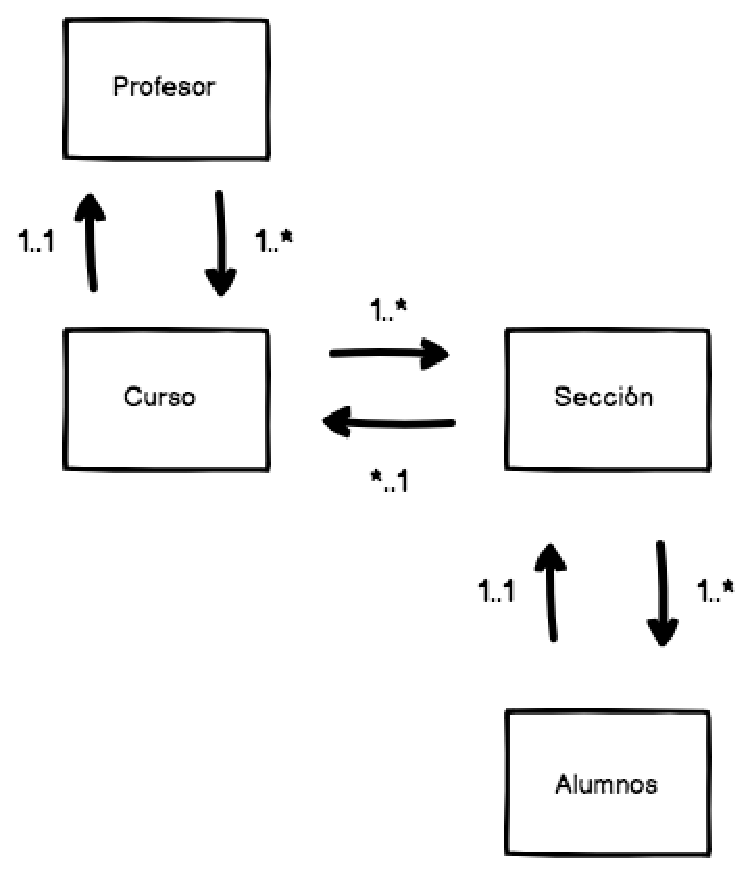
\includegraphics[width=0.4\textwidth]{images/base_de_datos.eps}
\caption{Esquema de la base de datos}
\label{fig:10}
\end{center}
\end{figure}

Como se muestra en la imagen, la estructura de la base de datos se divide en cuatro tablas:

\begin{itemize}
    \item Profesor: donde se almacena toda la información referente a los profesores que se registren en la plataforma.
    \item Curso: creados por el profesorado, se guarda la información detallada del curso (título, descripción, etc.).
    \item Sección: se podría definir como el lugar de realización del curso, como por ejemplo ``Arona'', que tiene registrados a los alumnos con sus resultados en el mismo.
    \item Alumno: tabla en la que se almacenan los datos, así como los resultados, de los estudiantes que realizan los cursos o talleres de pensamiento computacional.
\end{itemize}

%++++++++++++++++++++++++++++++++++++++++++++++++++++++++++++++++++++++++++++++

\subsection{Gemas utilizadas}
\label{1:sec:2}

Una de las funcionalidades y características que tiene Ruby, el lenguaje usado para desarrollar el proyecto, es la incorporación de gemas, al igual que ocurre con el entorno NodeJS y sus paquetes ``npm''.

CodeCharts posee algunas relevantes como:

\begin{itemize}
    \item \textbf{Rails}, la gema que incluye Ruby on Rails por defecto para la utilización del framework.
    \item \textbf{SQLite}\cite{SQLite}, para el manejo de las bases de datos, así como ActiveRecord.
    \item \textbf{Devise}\cite{Devise}, que ofrece una solución flexible para la autenticación de los usuarios en la aplicación.
    \item \textbf{Bootstrap}\cite{BootstrapGem}, gema que permite el diseño del front-end de la plataforma con Bootstrap.
    \item \textbf{Will-paginate}\cite{Paginate}, de manera que si hay una gran cantidad de usuarios dentro de una sección, permita agruparlos en páginas.
    \item \textbf{Wicked-pdf}\cite{WickedPDF}, con lo que el profesor puede descargar en formato .PDF los resultados de los alumnos.
    \item \textbf{Chartkick}, herramienta que muestra en forma gráfica los resultados obtenidos en los test de los estudiantes.
    \item \textbf{Jquery-rails}\cite{JqueryRails}, que incluye Jquery en la aplicación. 
\end{itemize}

%++++++++++++++++++++++++++++++++++++++++++++++++++++++++++++++++++++++++++++++

\section{Diseño de la aplicación}
\label{1:sec:2}

\subsection{Página de inicio}
\label{1:sec:1}

La primera vez que se accede a la aplicación, el profesor, que será el usuario a registrarse en la plataforma, verá una descripción de en qué consiste la aplicación y lo que ofrece al profesorado en los cursos impartidos.

\begin{figure}[!th]
\begin{center}
\includegraphics[width=0.5\textwidth]{images/captura_inicio.eps}
\label{fig:11}
\end{center}
\end{figure}

Dentro de está página, el profesor se podrá registrar por primera vez, o por el contrario, si ya dispone de una cuenta creada previamente, puede entrar con la misma.

%++++++++++++++++++++++++++++++++++++++++++++++++++++++++++++++++++++++++++++++

\subsection{Registro/Inicio de sesión}
\label{1:sec:2}

En las capturas que se observan a continuación, el profesor puede tanto crearse una cuenta, como iniciar con una ya creada, si ya se ha registrado previamente. 
\begin{figure}[!th]%
    \centering
    \subfloat{{\includegraphics[width=5cm]{images/registro.eps} }}%
    \qquad
    \subfloat{{\includegraphics[width=5cm]{images/inicio_sesion.eps} }}%
    \caption{Registro e inicio de sesión}%
    \label{fig:12}%
\end{figure}

El formulario de \textbf{creación de usuario} para la plataforma es muy sencillo, dado que consta de los datos básicos que se solicitan en la gran mayoría de páginas, como su nombre y apellidos, su correo electrónico y una contraseña.

%++++++++++++++++++++++++++++++++++++++++++++++++++++++++++++++++++++++++++++++

\subsection{Cursos creados}
\label{1:sec:3}

Una vez que el profesor ha accedido a la plataforma por primera vez, se mostrará una página como la que se observa en la figura. En ella se puede observar que se le informa al usuario que no tiene creado ningún curso/taller para sus alumnos, 
con lo que puede crearlos a través del botón de la parte superior izquierda.

\newpage
\begin{figure}[!th]
\begin{center}
\includegraphics[width=0.5\textwidth]{images/captura_cursos.eps}
\label{fig:13}
\end{center}
\end{figure}

Los cursos creados se irán mostrando al profesor en forma de cuadrícula, de manera que el tutor sepa los cursos que tiene creados, con su información asociada (título, descripción y fecha de creación).

\begin{figure}[!th]
\begin{center}
\includegraphics[width=0.5\textwidth]{images/cursos_creados.eps}
\label{fig:14}
\end{center}
\end{figure}

%++++++++++++++++++++++++++++++++++++++++++++++++++++++++++++++++++++++++++++++

\subsection{Perfil del profesor}
\label{1:sec:4}

Al profesor que haya iniciado sesión en ese momento, se le permitirá la opción de editar su perfil, a la vez que borrar su cuenta en caso de que ya no vaya a usar su cuenta en la plataforma.
Para que cualquier cambio, como se informa en el formulario, es necesaria la contraseña actual.

\begin{figure}[!th]
\begin{center}
\includegraphics[width=0.4\textwidth]{images/editar_perfil.eps}
\label{fig:15}
\end{center}
\end{figure}

%++++++++++++++++++++++++++++++++++++++++++++++++++++++++++++++++++++++++++++++

\subsection{Detalles del curso}
\label{1:sec:5}

En el momento que el docente cree el curso o taller, podrá acceder para observar los detalles del mismo, así como crear secciones dentro de la actividad.

\begin{figure}[!th]
\begin{center}
\includegraphics[width=0.5\textwidth]{images/detalles_curso.eps}
\label{fig:16}
\end{center}
\end{figure}

Al igual que con la página de las actividades, se le comunica al profesor que para observar las estadísticas de ese curso, tiene que añadir el lugar (Sección) donde se celebró el taller.
Uno de los detalles a destacar en el curso sería el de "Valor de referencia", que se podría definir como un número representativo que indica el nivel que tienen los alumnos de media que realizan
esa actividad.

\begin{figure}[!th]
\begin{center}
\includegraphics[width=0.5\textwidth]{images/curso_secciones.eps}
\label{fig:17}
\end{center}
\end{figure}

En la captura anterior se puede observar un curso creado de ejemplo, junto con las secciones donde se realizó el curso. Tiene tanto la posibilidad de administrar a los alumnos, como se muestra en el botón derecha, al igual que eliminarlo.

%++++++++++++++++++++++++++++++++++++++++++++++++++++++++++++++++++++++++++++++

\newpage
\subsection{Detalles de la sección}
\label{1:sec:6}

El objetivo final de la plataforma es que el profesor, cuando inserte los resultados de los alumnos obtenidos de la plataforma Code.org, observe con gráficos las calificaciones de cada uno.

\begin{figure}[!th]
\begin{center}
\includegraphics[width=0.7\textwidth]{images/lista_sin_alumnos.eps}
\label{fig:18}
\end{center}
\end{figure}

\begin{figure}[!th]
\begin{center}
\includegraphics[width=0.3\textwidth]{images/insertar_alumnos.eps}
\label{fig:19}
\end{center}
\end{figure}

Se pueden registrar alumnos en la plataforma tanto de manera manual (de uno en uno), como a través de un fichero .json con la información requerida, entre la que se encuentra el nombre, apellidos, edad, etc. Entre los datos más relevantes,
los niveles completados en ese reto, así como las líneas de código utilizadas en total.

\begin{figure}[!th]
\begin{center}
\includegraphics[width=0.7\textwidth]{images/subir_fichero.eps}
\label{fig:20}
\end{center}
\end{figure}

\newpage
Al finalizar los retos por parte de los alumnos, el profesor obtendrá una tabla con toda la información de cada uno paginados, de manera que la tabla no se vuelva muy extensa al matricular a muchos alumnos, como se muestra a continuación.

\begin{figure}[!th]
\begin{center}
\includegraphics[width=0.7\textwidth]{images/tabla_alumnos.eps}
\label{fig:21}
\end{center}
\end{figure}

Por otro lado, en el apartado de \textbf{estadísticas}, se mostrarán gráficos desarrollados con la intención de ver en qué nivel se fomenta el aprendizaje en los alumnos.

\begin{figure}[!th]
\begin{center}
\includegraphics[width=0.7\textwidth]{images/estadisticas_seccion.eps}
\label{fig:22}
\end{center}
\end{figure}

En la imagen anterior se pueden observar algunos de los resultados obtenidos en forma de gráficos por los alumnos en ese curso.
   
  %%%%%%%%%%%%%%%%%%%%%%%%%%%%%%%%%%%%%%%%%%%%%%%%%%%%%%%%%%%%%%%%%%%%%%%%%%%%%%%
  \newpage{\pagestyle{empty}}
  \thispagestyle{empty}
   
  \chapter{Verificación y pruebas}
  \label{chapter:cinco}
   
  %%%%%%%%%%%%%%%%%%%%%%%%%%%%%%%%%%%%%%%%%%%%%%%%%%%%%%%%%%%%%%%%%%%%%%%%%%%%%
% Chapter 5: Verificación y pruebas
%%%%%%%%%%%%%%%%%%%%%%%%%%%%%%%%%%%%%%%%%%%%%%%%%%%%%%%%%%%%%%%%%%%%%%%%%%%%%%%

En este capítulo se describen algunas de las pruebas realizadas para probar ciertos aspectos de la plataforma durante el desarrollo del proyecto, así como los problemas que se presentaron a la hora de realizar la aplicación.

%++++++++++++++++++++++++++++++++++++++++++++++++++++++++++++++++++++++++++++++

\section{Problemas encontrados}
\label{5:sec:1}

Durante el proceso de desarrollo del Trabajo Fin de Grado, surgieron diversos problemas para llevar a cabo la integración de la herramienta para la representación gráfica de los resultados de los alumnos.

En primer lugar, se decidió que la plataforma ``Code.org'' era la más completa al disponer de retos suficientes para los profesores, de manera que fomenten el aprendizaje del pensamiento computacional. A través de su repositorio en Github, donde
se aloja toda la página, se realizó un estudio para comprobar de qué manera estaba estructurada la página y posteriormente se procedió a intentar realizar la contribución.

Al comprobar que su estructura se actualizaba constantemente en el repositorio y era imposible integrar la herramienta, se diseñó un servicio web externo. Este servicio, como se explica en puntos anteriores, 
funciona de manera similar a Code.org, con la particularidad de que se añade la información de los alumnos una vez hayan finalizado el curso en el lugar (sección) que se esté realizando.

%++++++++++++++++++++++++++++++++++++++++++++++++++++++++++++++++++++++++++++++

\section{Testeo de la aplicación}
\label{5:sec:2}

Como se describió en el apartado de ``Tecnología utilizada'', las pruebas se realizaron con RSpec. Las pruebas se ejecutaron sobre alguno de los modelos de la aplicación:

\begin{itemize}
    \item \textbf{Curso}: se validan que los atributos que se le pasan al curso de ejemplo son correctos. A su vez, si un curso tiene una o más secciones, así como insertar cursos en la aplicación.
    \begin{figure}[!th]
    \begin{center}
    \includegraphics[width=0.6\textwidth]{images/pruebas_curso.eps}
    \caption{Pruebas realizadas al modelo de cursos}
    \label{fig:23}
    \end{center}
    \end{figure}
    
    \item \textbf{Sección}: para este modelo se comprueba que, tanto las secciones como los usuarios en las mismas, se crean correctamente, de igual manera que se pueden eliminar los usuarios.
    \begin{figure}[!th]
    \begin{center}
    \includegraphics[width=0.6\textwidth]{images/pruebas_seccion.eps}
    \caption{Pruebas realizadas al modelo de las secciones}
    \label{fig:24}
    \end{center}
    \end{figure}
    \item \textbf{Usuarios}: al igual que con la sección, se valida que se pueden introducir manualmente con éxito.
\end{itemize}

\newpage
Por último, como se observa en la imagen, una vez que se ejecuta el comando ``rspec -fd'', nos muestra el título de cada una de las pruebas y en la parte inferior la cantidad de pruebas que se realizaron
y, en caso de errores, nos lo indicaría. En este caso, todas las pruebas pasan correctamente.

\begin{figure}[!th]
\begin{center}
\includegraphics[width=0.5\textwidth]{images/resultado_pruebas.eps}
\caption{Resultado de los tests ejecutados}
\label{fig:25}
\end{center}
\end{figure}
   
  %%%%%%%%%%%%%%%%%%%%%%%%%%%%%%%%%%%%%%%%%%%%%%%%%%%%%%%%%%%%%%%%%%%%%%%%%%%%%%%
  \newpage{\pagestyle{empty}}
  \thispagestyle{empty}
   
  \chapter{Conclusiones y líneas futuras}
  \label{chapter:conclusiones}
   
  %%%%%%%%%%%%%%%%%%%%%%%%%%%%%%%%%%%%%%%%%%%%%%%%%%%%%%%%%%%%%%%%%%%%%%%%%%%%%
% Chapter 6: Conclusiones y líneas futuras
%%%%%%%%%%%%%%%%%%%%%%%%%%%%%%%%%%%%%%%%%%%%%%%%%%%%%%%%%%%%%%%%%%%%%%%%%%%%%%%

%---------------------------------------------------------------------------------

La plataforma desarrollada, llamada CodeCharts, pretende facilitar al profesorado la visualización del progreso de sus alumnos, de manera que una vez que los estudiantes hayan realizado los retos, puedan comprobar en qué medida los cursos
o talleres están ayudando en el fomento del pensamiento computacional a la hora de afrontar las actividades.

Una de las peculiaridades de esta aplicación es que está pensada para que solo la use el personal de la docencia, por ello se ha desarrollado para su uso de la manera más sencilla y cómoda. En el momento que el profesor disponga de todos los datos de los alumnos,
sólo debe proceder a introducirlos en la web, y ya podrá disfrutar de la funcionalidad que lo define, las estadísticas.

Algunas de las asignaturas cursadas en el itinerario de ``Tecnologías de la Información'' han contribuido a la realización del Trabajo Fin de Grado, lo que me ha facilitado su desarrollo y me ha permitido conocer nuevas tecnologías relacionadas con la creación de webs.

En cuanto a las líneas futuras del proyecto, existen algunas tareas pendientes que mejorar en CodeCharts, ya que no se han podido implementar o desarrollar en el plazo estipulado.

\begin{itemize}
    \item Creación de cuenta tanto para los profesores como para los alumnos. Como esta diseñado actualmente está pensado para que solo los profesores sean los encargados de recabar toda la información de los cursos. Los estudiantes podrían entrar
    con su cuenta para comprobar de igual manera que los profesores las estadísticas de los retos que han realizado, de manera que haya una interacción profesor-alumno más cercana.
    \item Datos almacenados en Code.org. Como se detallaba en puntos anteriores, la idea principal era implementar las estadísticas en la plataforma Code.org. Al no conseguirlo, se podrían obtener los resultados de los talleres realizados en la plataforma de Code.org, 
    de manera que el profesor pueda insertarlos directamente en CodeCharts.
\end{itemize}





   
  %%%%%%%%%%%%%%%%%%%%%%%%%%%%%%%%%%%%%%%%%%%%%%%%%%%%%%%%%%%%%%%%%%%%%%%%%%%%%%%
  \newpage{\pagestyle{empty}}
  \thispagestyle{empty}
   
  \chapter{Summary and conclusions}
  \label{chapter:ingles}
   
  %%%%%%%%%%%%%%%%%%%%%%%%%%%%%%%%%%%%%%%%%%%%%%%%%%%%%%%%%%%%%%%%%%%%%%%%%%%%%
% Chapter 7: Summary and conclusions
%%%%%%%%%%%%%%%%%%%%%%%%%%%%%%%%%%%%%%%%%%%%%%%%%%%%%%%%%%%%%%%%%%%%%%%%%%%%%%%

%++++++++++++++++++++++++++++++++++++++++++++++++++++++++++++++++++++++++++++++

The developed platform, called CodeCharts, aims to make it easier for teachers to visualize the progress of their students, so that once the students have made the challenges, they can see if the courses or workshops are helping in the future promotioning computational thinking when facing activities.

One of the features of this application is that it is designed so that it is only used by the teaching staff, for that reason it has been developed for its use in the most simple and comfortable way. When the teacher has all the students data, he just has to proceed to introduce them on the web, and you can enjoy the functionality that defines it, the statistics.

Regarding the future lines of the project, there are some pending tasks to improve in CodeCharts, since they could not be implemented or developed within the stipulated period.

\begin{itemize}
    \item Creating an account for both teachers and students. As it is currently designed, it is designed so that only teachers are the only one able to gather all the information of the courses. The students could enter with their account to verify in the same way that the teachers do with the statistics of the challenges they have made, so that there is a closer teacher-student interaction.
    \item Data stored in Code.org. As detailed in previous points, the main idea was to implement statistics on the Code.org platform. By failing to do this, the results of the workshops carried out on the Code.org platform could be obtained, so that the teacher can insert them directly into CodeCharts.
    \item Some of the subjects studied in the itinerary of ``Information Technologies'' have contributed to complete the Final Degree Project, which has made easier the development and has allowed me to know new technologies related to the creation of websites.
\end{itemize}


   
  %%%%%%%%%%%%%%%%%%%%%%%%%%%%%%%%%%%%%%%%%%%%%%%%%%%%%%%%%%%%%%%%%%%%%%%%%%%%%%%
  \newpage{\pagestyle{empty}}
  \thispagestyle{empty}
   
  \chapter{Presupuesto}
  \label{chapter:Presupuesto}
   
  %%%%%%%%%%%%%%%%%%%%%%%%%%%%%%%%%%%%%%%%%%%%%%%%%%%%%%%%%%%%%%%%%%%%%%%%%%%%%
% Chapter 8: Presupuesto
%%%%%%%%%%%%%%%%%%%%%%%%%%%%%%%%%%%%%%%%%%%%%%%%%%%%%%%%%%%%%%%%%%%%%%%%%%%%%%%

\section{Presupuesto}
\label{5:sec:2}

A continuación, se muestra el presupuesto que se estima para llevar a cabo la realización del proyecto.

%--------------------------------------------------------------------------
\begin{table}[!ht]
\begin{center}
\begin{tabular}{|p{60mm}|p{20mm}|p{40mm}|p{25mm}|} \hline 
\textbf{Recurso} & \textbf{Horas} & \textbf{Precio unidad} & \textbf{Total}\\ \hline
Estudio Pensamiento Computacional & 50 & 12\euro & 600\euro \\ \hline

Tutorial Ruby on Rails & 10 & 12\euro & 120\euro \\ \hline

Desarrollo de plataforma & 10 & 10\euro & 100\euro \\ \hline

Front-End & 50 & 12\euro & 600\euro \\ \hline

Back-End & 60 & 12\euro & 720\euro \\ \hline

Total & 170 & - &  \\ \hline

\end{tabular}
\end{center}
\caption{Tabla resumen del presupuesto}
\label{table:resOthers}
\end{table}


  %%%%%%%%%%%%%%%%%%%%%%%%%%%%%%%%%%%%%%%%%%%%%%%%%%%%%%%%%%%%%%%%%%%%%%%%%%%%%%%
  %\newpage{\pagestyle{empty}}
  %\thispagestyle{empty}
  %\begin{appendix}
   
  %\chapter{Título del Apéndice 1}
  %\label{appendix:1}
  %\input{apendice1.tex}
   
  %\chapter{Título del Apéndice 2}
  %\label{appendix:2}
  %\input{apendice2.tex}
   
  %\end{appendix}
   
  %%%%%%%%%%%%%%%%%%%%%%%%%%%%%%%%%%%%%%%%%%%%%%%%%%%%%%%%%%%%%%%%%%%%%%%%%%%%%%%
  \addcontentsline{toc}{chapter}{Bibliografía}
  \bibliographystyle{plain}
   
  \bibliography{memtfg}
  %\nocite{*}
   
  %%%%%%%%%%%%%%%%%%%%%%%%%%%%%%%%%%%%%%%%%%%%%%%%%%%%%%%%%%%%%%%%%%%%%%%%%%%%%%%
   
  \end{document}